\section{Concept}\label{concept}

skizze wie dom rendering funktioniert oder auch nicht, da es ziemlich
uninteressant ist

\subsection{How}\label{how}

\subsubsection{Server}\label{server}

\subsubsection{Client}\label{client}

\begin{figure}[htbp]
\centering
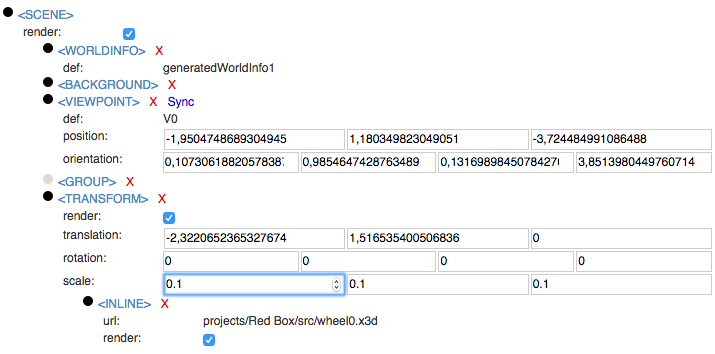
\includegraphics{../assets/treeview.png}
\caption{treeview}
\end{figure}

\paragraph{Synchronization Process}\label{synchronization-process}

\begin{quote}
``I conclude that there are two ways of constructing a software design:
One way is to make it so simple that there are obviously no deficiencies
and the other way is to make it so complicated that there are no obvious
deficiencies. The first method is far more difficult.\\
- Hoare, Turing Award Lecture 1980
\end{quote}

React is utilized by SceGraToo to render the tree-view-controller that
gives a more structured view of the scene-graph than the rendered scene.

The scene-graph is the most important part of SceGraToo, it shows the
the structure rather than the visual representation. Different
off-the-shelf solutions, like angular or JQuery plugins, were tested
against theses requirements:

\begin{enumerate*}
\def\labelenumi{\arabic{enumi}.}
\item
  custom html elements as part of tree nodes (multiple checkboxes or
  multiple inputs)
\item
  ability to observe the tree node's state changing
\item
  binding to an arbitrary model, that can recover inconsistent state
\end{enumerate*}

with mixed results:

\textbf{Partially not met requirements:}

\begin{itemize*}
\item
  custom elements as part of tree nodes
\item
  ability to listen to changes to the tree node
\end{itemize*}

\textbf{Requirements none of the tested tools met:}

\begin{itemize*}
\item
  binding to an arbitrary model, that can recover inconsistent views
\end{itemize*}

None of the off-the-shelf solutions could satisfy all expectations.

The most complicated part is keeping the tree-view-controller in sync
with the scene-graph while the scene-graph is being modified and vice
versa.

\subparagraph{Rerendering and Diffing}\label{rerendering-and-diffing}

Terminology

\textbf{scene-graph:}\\
The HTML/XML/X3D representation of the scene:

\begin{minted}[breaklines,bgcolor=bg]{html}
  <x3d version="3.0" profile="Interaction" width="708px" height="354px">
    <!-- id=69b81d54-6e7a-4967-acca-b8c89ba90782 -->
    <scene render="true" bboxcenter="0,0,0" bboxsize="-1,-1,-1" pickmode="idBuf" dopickpass="true">
      <worldinfo def="generatedWorldInfo1" title="Orgel" info="">
      </worldinfo>

      <background skycolor="0.3 0.3 0.3" groundcolor="" groundangle="" skyangle="" backurl="" bottomurl="" fronturl="" lefturl="" righturl="" topurl=""></background>

      <viewpoint def="V0" fieldofview="0.7" position="-1.9504748689304945 1.180349823049051 -3.724484991086488" orientation="0.10730618820578387 0.9854647428763489 0.13169898450784276 3.8513980449760714" centerofrotation="0 0 0" znear="-1" zfar="-1">
      </viewpoint>

      <!-- id=8d3f0a8a-b6d7-4acc-922b-ea59364443fa -->
      <group def="G1" render="true" bboxcenter="0,0,0" bboxsize="-1,-1,-1">
        <transform def="generatedTransform3" scale="1 1 1" rotation="0 0 1 0" translation="0 0 0" render="true" bboxcenter="0,0,0" bboxsize="-1,-1,-1" center="0,0,0" scaleorientation="0,0,0,0">
          <!-- id=8459b736-5a9d-4688-b624-e519857a92fd -->
          <inline def="O1_3" namespacename="O1_3" url="projects/Red Box/src/redBox.x3d" render="true" bboxcenter="0,0,0" bboxsize="-1,-1,-1" load="true">
            <Shape render="true" bboxCenter="0,0,0" bboxSize="-1,-1,-1" isPickable="true">
              <Appearance sortType="auto" alphaClipThreshold="0.1">
                <Material diffuseColor="1 0 0" ambientIntensity="0.2" emissiveColor="0,0,0" shininess="0.2" specularColor="0,0,0"></Material>
              </Appearance>
              <Box solid="true" ccw="true" useGeoCache="true" lit="true" size="2,2,2"></Box>
            </Shape>
          </inline>
        </transform>
      </group>
    </scene>
  </x3d>
\end{minted}


\textbf{tree-view-controller:}\\
Loosely defined term that comprises all objects, methods, functions,
event-listeners and callbacks related to parsing the scene-graph and
creating the initial tree-view-view.

\textbf{tree-view-node-controller:} Loosely defined term that comprises
all objects, methods, functions, event-listeners end callbacks related
to keeping a subtree of the scene-graph up to date.

\textbf{tree-view-view:}\\
The HTML representation of the tree-view-controller (html output
shortened and simplified):\\
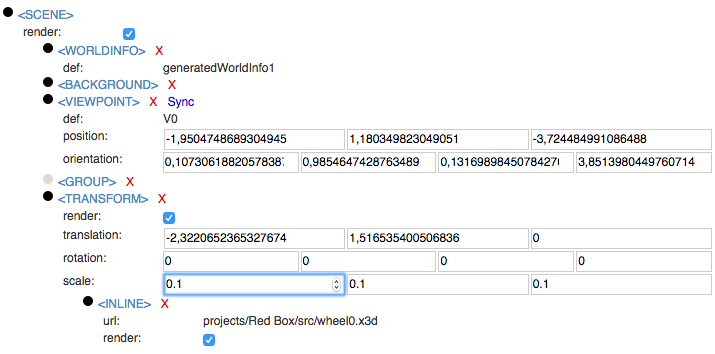
\includegraphics{../assets/treeview.png}

\begin{minted}[breaklines,bgcolor=bg]{html}
  <div>
    <li>
      <div>
        <div></div>
        <a>
          <span></span>
          <span>SCENE</span>
        </a>
      </div>
      <div>
        <div>
          <div>
            <div>
              <span>render</span>
              <span>:</span>
            </div>
            <div>
              <input type="checkbox">
            </div>
          </div>
        </div>
        <ol>
          <li>
            <div>
              <div></div>
              <a>
                <span></span>
                <span>WORLDINFO</span>
              </a><a>X</a></div>
            <div>
              <div>
                <div>
                  <div>
                    <span>def</span>
                    <span>:</span>
                  </div>
                  <div>generatedWorldInfo1</div>
                </div>
              </div>
              <ol></ol>
            </div>
  ...
        </ol>
      </div>
    </li>
  </div>
\end{minted}

The aim is to keep the tree-view-view a consistent representation of the
scene-graph. The tree-view-view only shows specific nodes, I can't list
them here because they will change over the

where specific scene-graph nodes, ones that , and their properties are
presented in an up to date and editable form.

todo: explain what nodes and what properties and why

First design approach is to let the tree-view-controller create an
initial tree-view-view by traversing it and creating
tree-view-node-controllers ad hoc. These tree-view-node-controllers
create the corresponding tree-view-node-views while traversing the
scene-graph. For each scene-graph node create a corresponding
tree-view-view node. Each tree-view-node-controller observes its
corresponding scene-graph node for attribute mutations and added or
removed child nodes and change it's view accordingly.

Depending on how the scene-graph is mutated 3 main cases can be
differentiated.

\begin{description*}
  \item a scene-graph node is added \hfill \\
    a new tree-view-node-controller is instantiated and renders a new tree-view-node-view
  \item a scene-graph node is deleted \hfill \\
    the corresponding tree-view-node-controller is destroyed
  \item a scene-graph node is mutated \hfill \\
    the corresponding tree-view-node-view is altered
\end{description*}

Tree-view-node-views can also be used to edit a scene-graph node's
properties.\\
When a tree-view-node-views is edited it's tree-view-node-controller is
notified and applies the new properties to the corresponding scene-graph
node. It's assumed that the updates will always lead to consistent
state, where the scene-graph and the tree node converge.

The synchronization process has no ability to detect if updates lead to
a consistent state. It also has no ability to recover from an
inconsistent state, though without the ability to detect inconsistencies
this does not really matter.

\textbf{Problem 1:} keeping the tree-view consistent with the
scene-graph\\
The difficulty to make sure that incremental updates are error-free
exacerbates even more when further functionality, like checkboxes for
specific properties or saving state in the tree-view that is not part of
the scene-graph, like the possibility to collapse parts of the tree , is
added to the tree-view.

\textbf{Problem 2:} implementation effort\\
For every new feature 4 things have to implemented:\\
\begin{enumerate}
  \item code for parsing the the scene-graph
  \item code to generate the tree-view-node-view
  \item code to synchronize changes from the scene-graph to the tree-view-node-view
  \item code to synchronize changes from the tree-view-node-view to the scene-graph
\end{enumerate}

This design bears more complexity than reparsing and regenerating the
complete tree-view-view on every change.

Rerendering solves Problem 1 and reduces problem 2 to two steps:\\
\begin{enumerate}
  \item code for parsing the scene-graph and generating the tree-view-node-view
  \item code to synchronize changes from the tree-view-node-view to the scene-graph
\end{enumerate}


Rerendering everything on every change is usually inefficient. React is
used to circumvent this problem. React calculates a lightweight
representation of what is going to be rendered to the DOM and compares
that to what is already rendered. It calculates a set of patches and
only applies these to the DOM.

The complete rerender of the view happens only im memory and is never
sent to the DOM and thus never

The code below is for explanation purposes and does not resemble react's
implementation in any way.

\textbf{Old Virtiual DOM:}

\begin{minted}[breaklines,bgcolor=bg]{html}
<ol data-reactid=".0">
  <li data-reactid=".0.0">scene
    <ol data-reactid=".0.0.0">
      <li data-reactid=".0.0.0.0">transform
        <ol data-reactid=".0.0.0.0.0">
          <li data-reactid=".0.0.0.0.0.0">inline</li>
        </ol>
      </li>
    </ol>
  </li>
</ol>
\end{minted}

\textbf{New Virtual DOM:}
\begin{minted}[breaklines,bgcolor=bg]{html}
<ol data-reactid=".0">
  <li data-reactid=".0.0">scene
    <ol data-reactid=".0.0.0">
      <li data-reactid=".0.0.0.0">transform
        <ol data-reactid=".0.0.0.0.0">
          <li data-reactid=".0.0.0.0.0.0">inline</li>
        </ol>
      </li>
      <li>group</li>
    </ol>
  </li>
</ol>
\end{minted}

\textbf{Patch:}

\begin{minted}[breaklines,bgcolor=bg]{javascript}
  var li = document.createElement('li')
  li.innerText = 'group'
  document.querySelector('[data-reactid=".0.0.0"]').appendChild(li)
\end{minted}

That means as long as the code that parses the scene-graph and generates
the lightweight representation is correct, the tree-view-view is
correct.

\subparagraph{Data Binding}\label{data-binding}

Another idea is to utilize templates and data binding. Frameworks like
{[}angular{]} or web components implementations like {[}polymer{]}
support templates and two way data binding. Following I'm just
concerning angular directives, but the same should be possible with web
components.

An angular directive consists of a mostly logic less template and some
javascript containing logic for creating the directive or reacting to
events.

For each node a directive is instantiated which creates a template
rendering the node. Also for each child it creates a new instance of
itself.

\textbf{Example:}

The \texttt{treenode} renders the node itself and a \texttt{nodelist},
that renders a list of tree-nodes for each child node. Mind the
recursion.

\begin{listing}[H]
\mint{cl}/(car (cons 1 '(2)))/
\caption{Example of a listing.}
\label{lst:example}
\end{listing}
Listing \ref{lst:example} contains an example of a listing.

The data:
\begin{listing}[H]
  \caption{Example of a listing.}
  \begin{minted}[breaklines,bgcolor=bg]{javascript}
  node: {
    name: "scene",
    children: [
      {
        name: "viewpoint"
      },
      {
        name: "worldinfo"
      }
    ]
  }
  \end{minted}
\end{listing}

\begin{minted}[breaklines,bgcolor=bg]{html}
  <treenode node="node">
  </treenode>
\end{minted}

\begin{minted}[breaklines,bgcolor=bg]{html}
  <treenode node="node">
    <span>{{node.name}}</span>
    <nodelist ng-repeat='node in children' children='children'>
    </nodelist>
  </treenode>
\end{minted}

\begin{minted}[breaklines,bgcolor=bg]{html}
  <treenode node="node">
    <span>{{node.name}}</span>
    <nodelist ng-repeat='node in children' children='children'>
      <treenode node="children[0]">
      </treenode>
      <treenode node="children[1]">
      </treenode>
    </nodelist>
  </treenode>
\end{minted}

\begin{minted}[breaklines,bgcolor=bg]{html}
  <treenode node="node">
    <span>{{node.name}}</span>
    <nodelist ng-repeat='node in children' children='children'>
      <treenode node="children[0]">
        <span>{{node.name}}</span>
      </treenode>
      <treenode node="children[1]">
        <span>{{node.name}}</span>
      </treenode>
    </nodelist>
  </treenode>
\end{minted}

Again, this is not an accurate depiction of how angular works, it's just
for illustration purposes.

The scene-graph is traversed and for each eligible child node a new
\texttt{treenode} is created. The double curly braces are angular's way
to denote data-binding in templates. The data from the elements scope is
automatically inserted and kept up to date. This data binding would then
ensure that when the scene-graphs attributes are changed the model is
kept in sync and the other way around.

\subsubsection{Interaction}\label{interaction}
